\documentclass[aspectratio=169]{beamer}
\usepackage{lmodern}
\usepackage{xcolor}
\usepackage[utf8]{inputenc}
\usepackage[english]{babel}

\usepackage{tikz}
\usetikzlibrary{shapes,arrows}

\usepackage[digital,srcmeas,semicon]{circdia}

\newcommand{\bluebox}[2] {
    \vfill
    \fcolorbox{red}{white}{\textcolor{red}{\textbf{#1 } #2}}
    }

\title{LibreSilicon's Standard Cell Library}
\subtitle{show and tell}
\author{chipforge}
\date{36c3} 

\begin{document}

% define block styles
\tikzstyle{decision} = [diamond, draw, text width=4.5em, text badly centered, node distance=3cm, inner sep=0pt]
\tikzstyle{block} = [rectangle, draw, text width=5em, text centered, rounded corners, minimum height=4em]
\tikzstyle{line} = [draw, -latex']
\tikzstyle{cloud} = [draw, ellipse, node distance=3cm, minimum height=2em]

%   ------------    title   -------------------------------------------

\begin{frame}
\titlepage
\end{frame}

%   ------------    disclaimer      -----------------------------------

\begin{frame}
\frametitle{disclaimer} 
This design is distributed in the hope that it will be useful, but
\textsc{WITHOUT ANY WARRANTY}; without even the implied warranty of
\textsc{MERCHANTABILITY} or \textsc{FITNESS FOR A PARTICULAR PURPOSE}.
\end{frame}

%   ------------    preview -------------------------------------------

%   list \section and \subsection, no frames

\begin{frame}
\frametitle{preview}
\tableofcontents
\end{frame}

%   ===================================================================
\section{LibreSilicon}
%   ===================================================================

%   ------------    History -------------------------------------------

\begin{frame}
\frametitle{LibreSilicon's History}
    \begin{itemize}
%       \setlength\itemsep{1em}
        \item 2017: Leviathanch finds a Clean Room at HKUST to rent
        \item Leviathanch gives a Lightning Talk at 34c3
        \item 2018: Developing a 1 Micron CMOS process
        \item Presenting current status at 35c3 with 1st Testwafer
        \item 2019: No money left for renting Clean Room further
        \item HKUST closed with Riots at Hong Kong
        \item Seeking for alternative Clean Rooms
    \end{itemize}

https://www.gofundme.com/f/libresilicon-cleanroom-rent
\end{frame}

%   ------------    URLs    -------------------------------------------

\begin{frame}
\frametitle{LibreSilicon's Standard Cell Library} 
https://libresilicon.com ($\rightarrow$ home page) \newline
https://www.github.com/chipforge/StdCellLib ($\rightarrow$ repository) \newline
https://vcs.in-berlin.de/chipforge\_stdcelllib/index ($\rightarrow$ wiki) \newline
\end{frame}

%   ------------    checkout    ---------------------------------------

\begin{frame}
\frametitle{checkout}
\texttt{\% git clone https://github.com/chipforge/StdCellLib.git StdCellLib}
\end{frame}

%   ===================================================================
\section{Basics}
%   ===================================================================

%   ------------    design flow ---------------------------------------

\begin{frame}
\frametitle{design flow}
    \begin{itemize}
%       \setlength\itemsep{1em}
        \item Write code in a Hardware Description Language like VHDL, Verilog or even SpinalHDL
        \item Simulate and verify the code
        \item 'compile' code into a Netlist $\rightarrow$ e.g. with 'Yosys'
        \item Netlist contains Gates, (Latches) and FlipFlops as Cells
        \item Cells are placed and routed in a Layout
        \item GDS II files for Mask production generated from Layout $\rightarrow$ 'Gerber' file format for Chips
    \end{itemize}

About the cells we are talking about here
\end{frame}

%   ------------    design goals    -----------------------------------

\begin{frame}{design goals}
    \begin{itemize}
%       \setlength\itemsep{1em}
        \item Get almost complete (more cells $\rightarrow$ better netlist)
        \item Less energy consuming (less Joule per Cell)
        \item As fast as possible (w/ small timing delay)
        \item Small footprint (small cell size)
    \end{itemize}
\end{frame}

%   ------------    nand2   -------------------------------------------

\begin{frame}
\frametitle{NAND2}
    \begin{figure}[h]
        \begin{center}
            \begin{circuitdiagram}{11}{6}
                \usgate
                \gate[\inputs{2}]{nand}{5}{3}{R}{}{NAND2}
                \pin{1}{1}{L}{A}    % pin A
                \pin{1}{5}{L}{A1}   % pin A1
                \pin{10}{3}{R}{Y}   % pin Y
            \end{circuitdiagram}
            \hspace{2cm}
            \begin{tabular}{ c c|c } 
                A1 & A & Y \\ 
                \hline
                0 & 0 & 1 \\ 
                0 & 1 & 1 \\ 
                1 & 0 & 1 \\ 
                1 & 1 & 0 \\ 
            \end{tabular}
        \end{center}
    $Y = \overline{ (A1 \cdot A) }$
    \end{figure}
\end{frame}

\begin{frame}
\frametitle{NAND2}
    \begin{figure}[h]
        \begin{center}
            \begin{circuitdiagram}{18}{20}
                \trans[\wireUD{0.5}]{penh*}{6}{16}{R}{}{}
                \pin{3}{17.5}{L}{A}
                \trans[\wireUD{0.5}]{penh*}{14}{16}{R}{}{}
                \pin{11}{17.5}{L}{A1}
                \power{8}{19}{U}{}
                \power{16}{19}{U}{}
                \trans[\wireUD{0.5}]{nenh*}{6}{10}{R}{}{}
                \pin{3}{8.5}{L}{A}
                \trans[\wireUD{0.5}]{nenh*}{6}{4}{R}{}{}
                \pin{3}{2.5}{L}{A1}
                \ground{8}{1}{D}
                \pin{17}{13}{R}{Y}
                \wire{8}{13}{16}{13}
                \wire{8}{13}{8}{13}
            \end{circuitdiagram}
        \end{center}
    \end{figure}
\end{frame}

%   ------------    nor2    -------------------------------------------

\begin{frame}
\frametitle{NOR2}
    \begin{figure}[h]
        \begin{center}
            \begin{circuitdiagram}{11}{6}
                \usgate
                \gate[\inputs{2}]{nor}{5}{3}{R}{}{NOR2}
                \pin{1}{1}{L}{A}    % pin A
                \pin{1}{5}{L}{A1}   % pin A1
                \pin{10}{3}{R}{Y}   % pin Y
            \end{circuitdiagram}
            \hspace{2cm}
            \begin{tabular}{ c c|c } 
                A1 & A & Y \\ 
                \hline
                0 & 0 & 1 \\ 
                0 & 1 & 0 \\ 
                1 & 0 & 0 \\ 
                1 & 1 & 0 \\ 
            \end{tabular}
        \end{center}
    $Y = \overline{ (A1 + A) }$
    \end{figure}
\end{frame}

\begin{frame}
\frametitle{NOR2}
    \begin{figure}[h]
        \begin{center}
            \begin{circuitdiagram}{18}{20}
                \trans[\wireUD{0.5}]{penh*}{6}{10}{R}{}{}
                \pin{3}{11.5}{L}{A}
                \trans[\wireUD{0.5}]{penh*}{6}{16}{R}{}{}
                \pin{3}{17.5}{L}{A1}
                 \power{8}{19}{U}{}
                \trans[\wireUD{0.5}]{nenh*}{6}{4}{R}{}{}
                \pin{3}{2.5}{L}{A}
                \trans[\wireUD{0.5}]{nenh*}{14}{4}{R}{}{}
                \pin{11}{2.5}{L}{A1}
                \ground{8}{1}{D}
                \ground{16}{1}{D}
                \pin{17}{7}{R}{Y}
                \wire{8}{7}{16}{7}
            \end{circuitdiagram}
        \end{center}
    \end{figure}
\end{frame}

%   ------------    xor2    -------------------------------------------

\begin{frame}
\frametitle{XOR2}
    \begin{figure}[h]
        \begin{center}
            \begin{circuitdiagram}{11}{6}
                \usgate
                \gate[\inputs{2}]{xor}{5}{3}{R}{}{XOR2}
                \pin{1}{1}{L}{A}    % pin A
                \pin{1}{5}{L}{A1}   % pin A1
                \pin{10}{3}{R}{Y}   % pin Y
            \end{circuitdiagram}
            \hspace{2cm}
            \begin{tabular}{ c c|c } 
                A1 & A & Y \\ 
                \hline
                0 & 0 & 0 \\ 
                0 & 1 & 1 \\ 
                1 & 0 & 1 \\ 
                1 & 1 & 0 \\ 
            \end{tabular}
        \end{center}
    $Y = A1 \oplus A$
    \end{figure}
There are a couple of different implementations known in literature.
\end{frame}

%   ------------    eq2     -------------------------------------------

\begin{frame}
\frametitle{EQ2}
    \begin{figure}[h]
        \begin{center}
            \begin{circuitdiagram}{11}{6}
                \usgate
                \gate[\inputs{2}]{xnor}{5}{3}{R}{}{EQ2}
                \pin{1}{1}{L}{A}    % pin A
                \pin{1}{5}{L}{A1}   % pin A1
                \pin{10}{3}{R}{Y}   % pin Y
            \end{circuitdiagram}
            \hspace{2cm}
            \begin{tabular}{ c c|c } 
                A1 & A & Y \\ 
                \hline
                0 & 0 & 1 \\ 
                0 & 1 & 0 \\ 
                1 & 0 & 0 \\ 
                1 & 1 & 1 \\ 
            \end{tabular}
        \end{center}
    $Y = \overline{ (A1 \oplus A) }$
    \end{figure}
Same as for XOR2, different implementations known in literature.
\end{frame}

%   ------------    complex gates   -----------------------------------

\begin{frame}
\frametitle{complex gates}
    \begin{figure}[h]
        \begin{center}
            \begin{circuitdiagram}{18}{8}
                \usgate
                \gate[\inputs{2}]{and}{5}{5}{R}{}{}  % AND
                \gate[\inputs{2}]{nor}{12}{3}{R}{}{} % NOR
                \pin{1}{1}{L}{A}    % pin A
                \pin{1}{3}{L}{B}    % pin B
                \pin{1}{7}{L}{B1}   % pin B1
                \wire{2}{1}{9}{1}   % wire from pin A
                \pin{17}{3}{R}{$Y_{AOI21}$}   % pin Y
            \end{circuitdiagram}
            \hspace{2cm}
            \begin{circuitdiagram}{18}{8}
                \usgate
                \gate[\inputs{2}]{or}{5}{5}{R}{}{}  % OR
                \gate[\inputs{2}]{nand}{12}{3}{R}{}{} % NAND
                \pin{1}{1}{L}{A}    % pin A
                \pin{1}{3}{L}{B}    % pin B
                \pin{1}{7}{L}{B1}   % pin B1
                \wire{2}{1}{9}{1}   % wire from pin A
                \pin{17}{3}{R}{$Y_{OAI21}$}   % pin Y
            \end{circuitdiagram}
        \end{center}
    $Y_{AOI21} = \overline{ ((B1 \cdot B ) + A) }$
    \hspace{2cm}
    $Y_{OAI21} = \overline{ ((B1 + B ) \cdot A) }$
    \end{figure}

    \begin{figure}[h]
        \begin{center}
            \begin{circuitdiagram}{18}{12}
                \usgate
                \gate[\inputs{2}]{and}{5}{9}{R}{}{}  % AND
                \gate[\inputs{2}]{and}{5}{3}{R}{}{}  % AND
                \gate[\inputs{2}]{nor}{12}{6}{R}{}{} % NOR
                \pin{1}{1}{L}{A}     % pin A
                \pin{1}{5}{L}{A1}    % pin A1
                \pin{1}{7}{L}{B}     % pin B
                \pin{1}{11}{L}{B1}   % pin B1
                \wire{9}{3}{9}{4}    % wire between AND and NOR
                \wire{9}{9}{9}{8}    % wire between AND and NOR
                \pin{17}{6}{R}{$Y_{AAOI22}$}   % pin Y
            \end{circuitdiagram}
            \hspace{2cm}
            \begin{circuitdiagram}{18}{12}
                \usgate
                \gate[\inputs{2}]{or}{5}{9}{R}{}{}    % OR gate -> right
                \gate[\inputs{2}]{or}{5}{3}{R}{}{}    % OR gate -> right
                \gate[\inputs{2}]{nand}{12}{6}{R}{}{}    % NAND gate -> right
                \pin{1}{1}{L}{A0}    % pin A0
                \pin{1}{5}{L}{A1}    % pin A1
                \pin{1}{7}{L}{B}     % pin B
                \pin{1}{11}{L}{B1}   % pin B1
                \wire{9}{3}{9}{4}    % wire between OR and NAND 
                \wire{9}{9}{9}{8}    % wire between OR and NAND 
                \pin{17}{6}{R}{$Y_{OOAI22}$}   % pin Y
            \end{circuitdiagram}
        \end{center}
    $Y_{AAOI22} = \overline{ ((B1 \cdot B) + (A1 \cdot A)) }$
    \hspace{2cm}
    $Y_{OOAI21} = \overline{ ((B1 + B) \cdot (A1 + A)) }$
    \end{figure}
How far we can go?
\end{frame}

%   ------------    design considerations   ---------------------------

\begin{frame}
\frametitle{design considerations}
    \begin{figure}[h]
        \begin{center}
            \begin{circuitdiagram}{50}{33}
                \pin{2}{2.5}{L}{A3}  % pin A3
                \pin{2}{8.5}{L}{A2}  % pin A2
                \pin{2}{14.5}{L}{A1} % pin A1
                \pin{2}{20.5}{L}{A} % pin A
                \pin{2}{29.5}{L}{A}  % pin A
                \pin{14}{29.5}{L}{A1} % pin A1
                \pin{26}{29.5}{L}{A2} % pin A2
                \pin{38}{29.5}{L}{A3} % pin A3
                \trans[\wireUD{0.5}]{nenh*}{6}{4}{R}{}{}
                \trans[\wireUD{0.5}]{nenh*}{6}{10}{R}{}{}
                \trans[\wireUD{0.5}]{nenh*}{6}{16}{R}{}{}
                \trans[\wireUD{0.5}]{nenh*}{6}{22}{R}{}{}
                \trans[\wireUD{0.5}]{nenh*}{54}{22}{R}{}{}
                \trans[\wireUD{0.5}]{penh*}{6}{28}{R}{}{}
                \trans[\wireUD{0.5}]{penh*}{18}{28}{R}{}{}
                \trans[\wireUD{0.5}]{penh*}{30}{28}{R}{}{}
                \trans[\wireUD{0.5}]{penh*}{42}{28}{R}{}{}
                \trans[\wireUD{0.5}]{penh*}{54}{28}{R}{}{}
                \ground{8}{0.5}{D}  % ground below nmos
                \ground{56}{18.5}{D}  % ground below inverter
                \power{8}{31.5}{U}{}  % power above left pmos
                \power{20}{31.5}{U}{}  % power above middle pmos
                \power{32}{31.5}{U}{}  % power above middle pmos
                \power{44}{31.5}{U}{}  % power above right pmos
                \power{56}{31.5}{U}{}  % power above inverter
                \wire{8}{25}{51}{25}    % wire before inverter gate
                \junct{8}{25}
                \junct{20}{25}
                \junct{32}{25}
                \junct{44}{25}
                \junct{56}{25}
                \wire{51}{29.5}{51}{20.5}   % wire at inverter gates
                \junct{51}{25}
                \wire{56}{25}{58}{25}    % wire before pin Z
                \pin{59}{25}{R}{Z}  % pin Z
            \end{circuitdiagram}
        \end{center}
    \end{figure}
\end{frame}

\begin{frame}
\frametitle{design considerations}
    \begin{itemize}
%       \setlength\itemsep{1em}
        \item 2 stacked transistors $\rightarrow$ library to small
        \item 3 stacked transistors $\rightarrow$ quite common for small nodes
        \item 4 stacked transistors $\rightarrow$ huge library
        \item buffer limit $\ge$ 3 transistors
    \end{itemize}
\end{frame}

%   ------------    cell enlargement    -------------------------------

\begin{frame}
\frametitle{cell enlargement}
    \begin{itemize}
%       \setlength\itemsep{1em}
        \item add transistor into pull-up (or pull-down) network in serial
        \item add complementary transistor in parallel
    \end{itemize}
\end{frame}

%   ------------    nor2    -------------------------------------------

\begin{frame}
\frametitle{NOR2}
    \begin{center}
        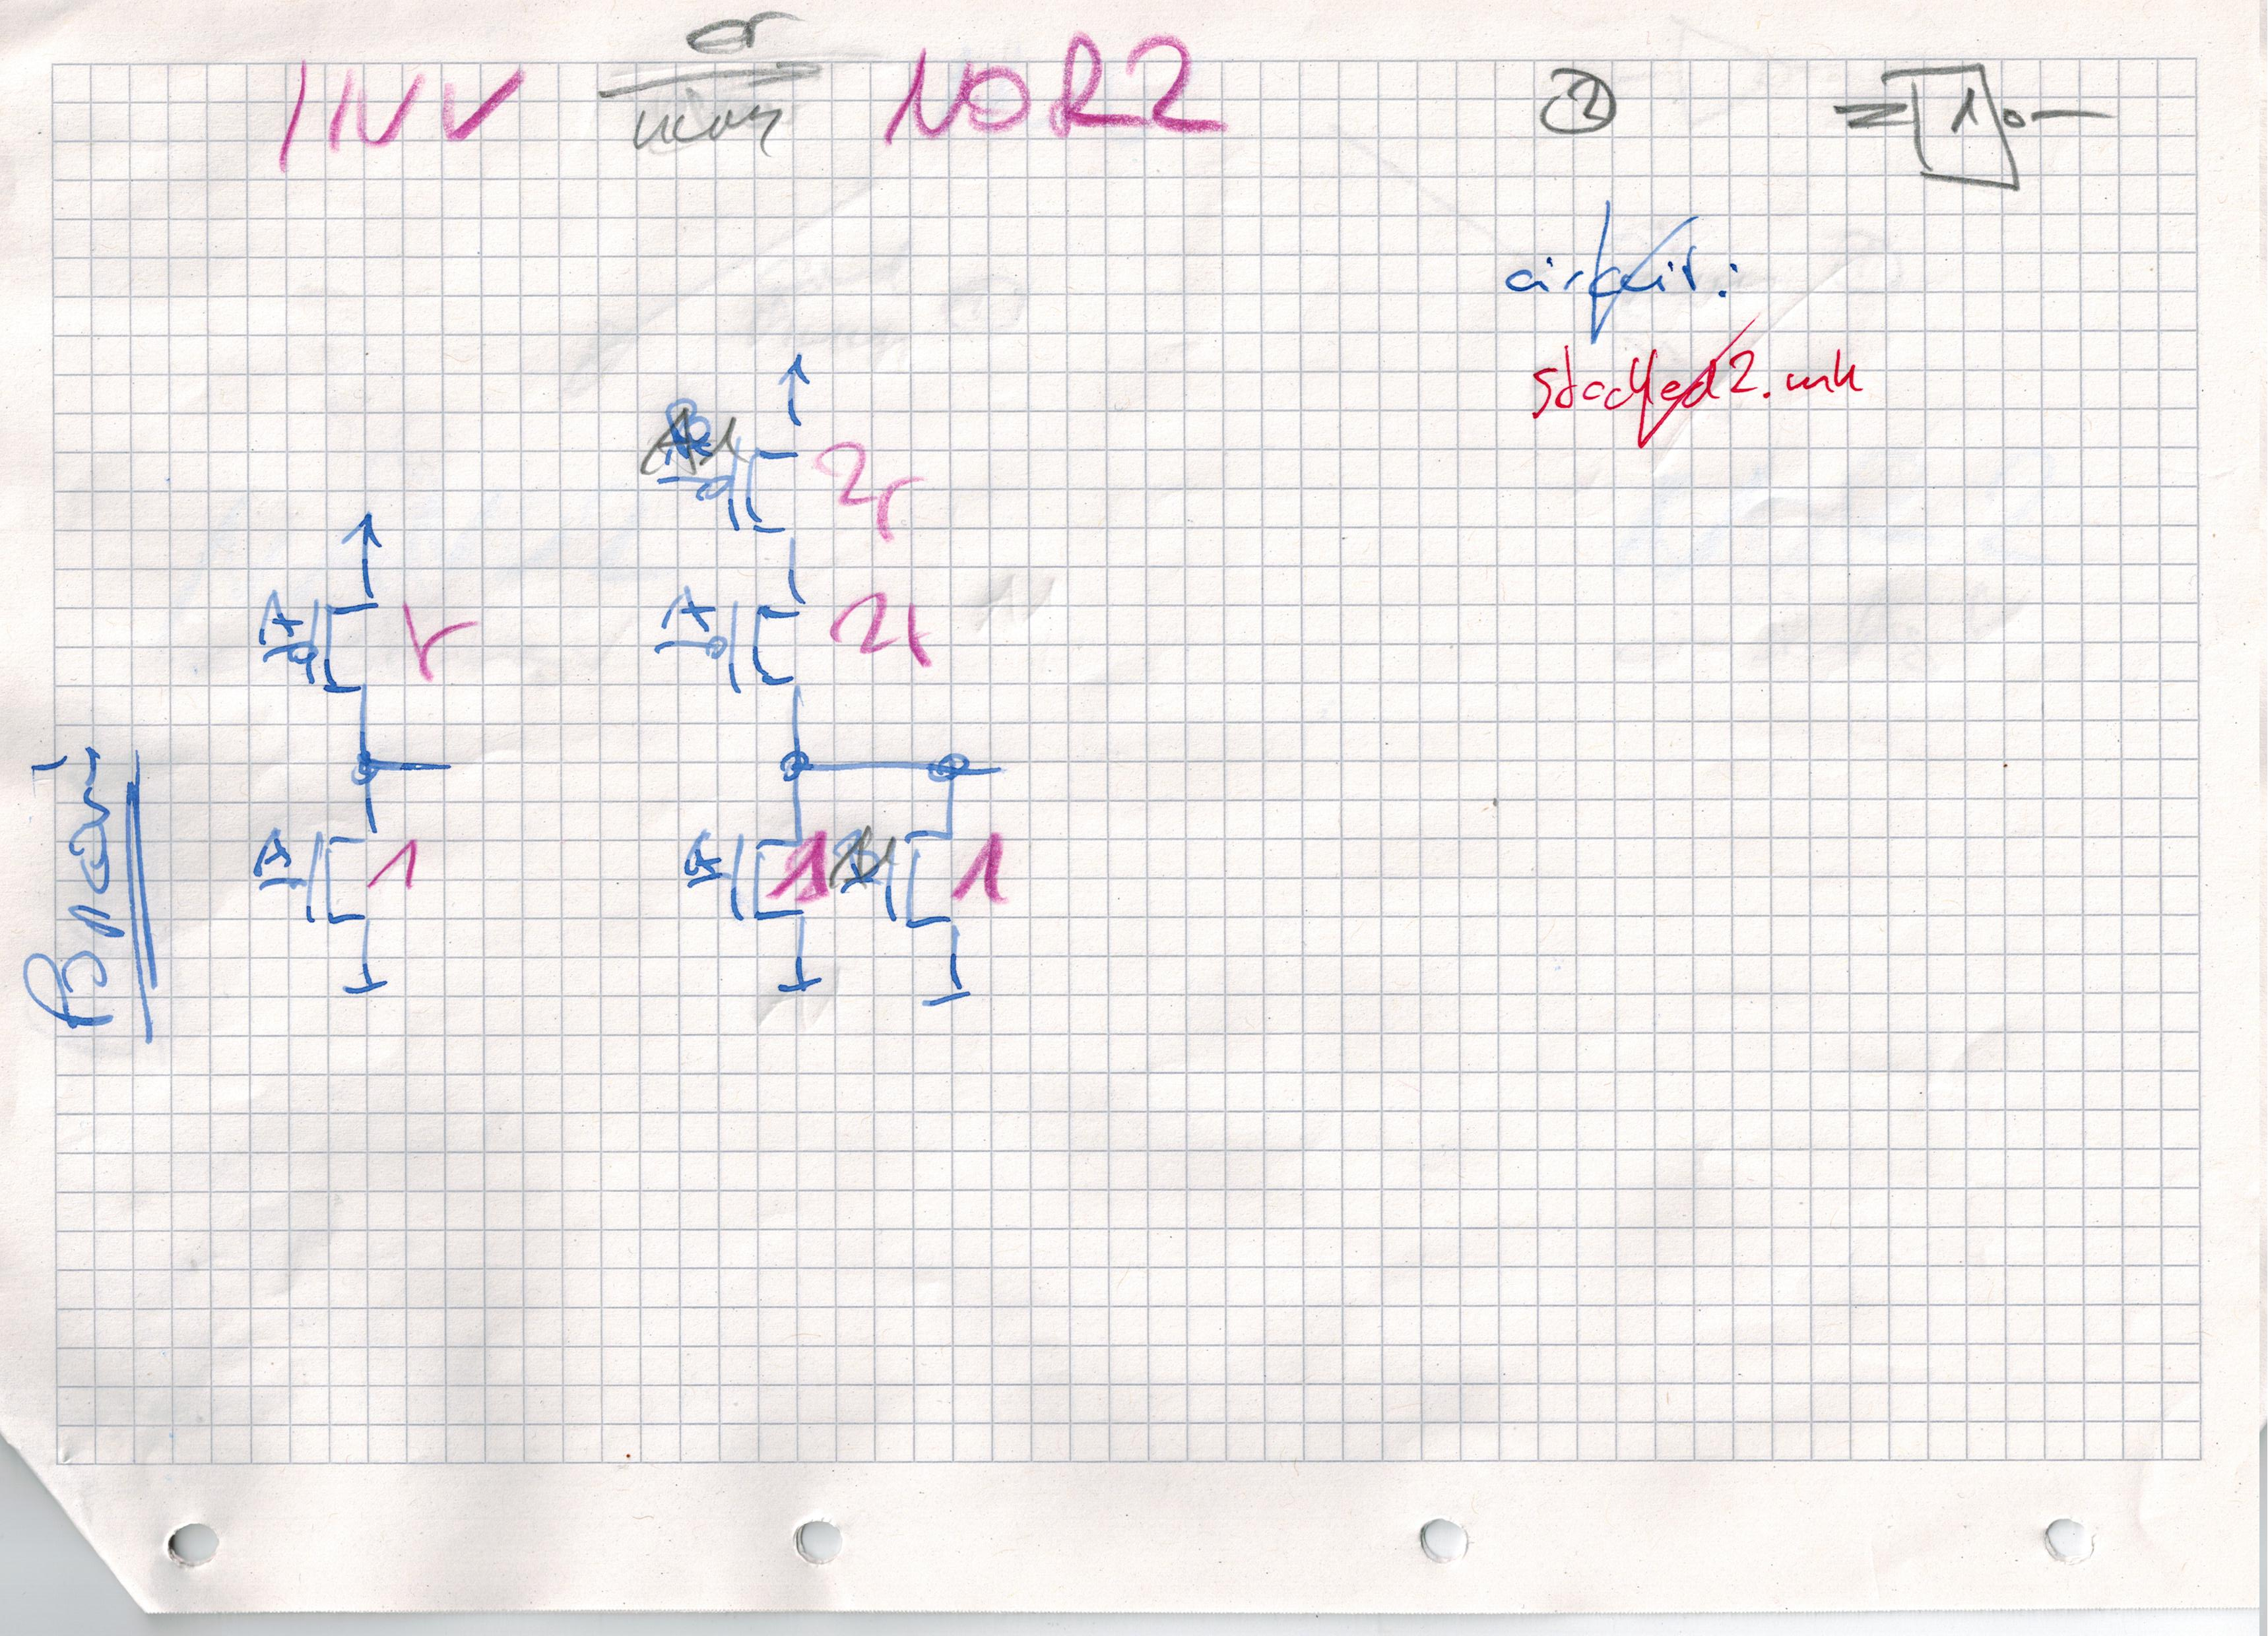
\includegraphics[width=0.85\textwidth]{NOR2.jpg}
    \end{center}
\end{frame}

%   ------------    nand2   -------------------------------------------

\begin{frame}
\frametitle{NAND2}
    \begin{center}
        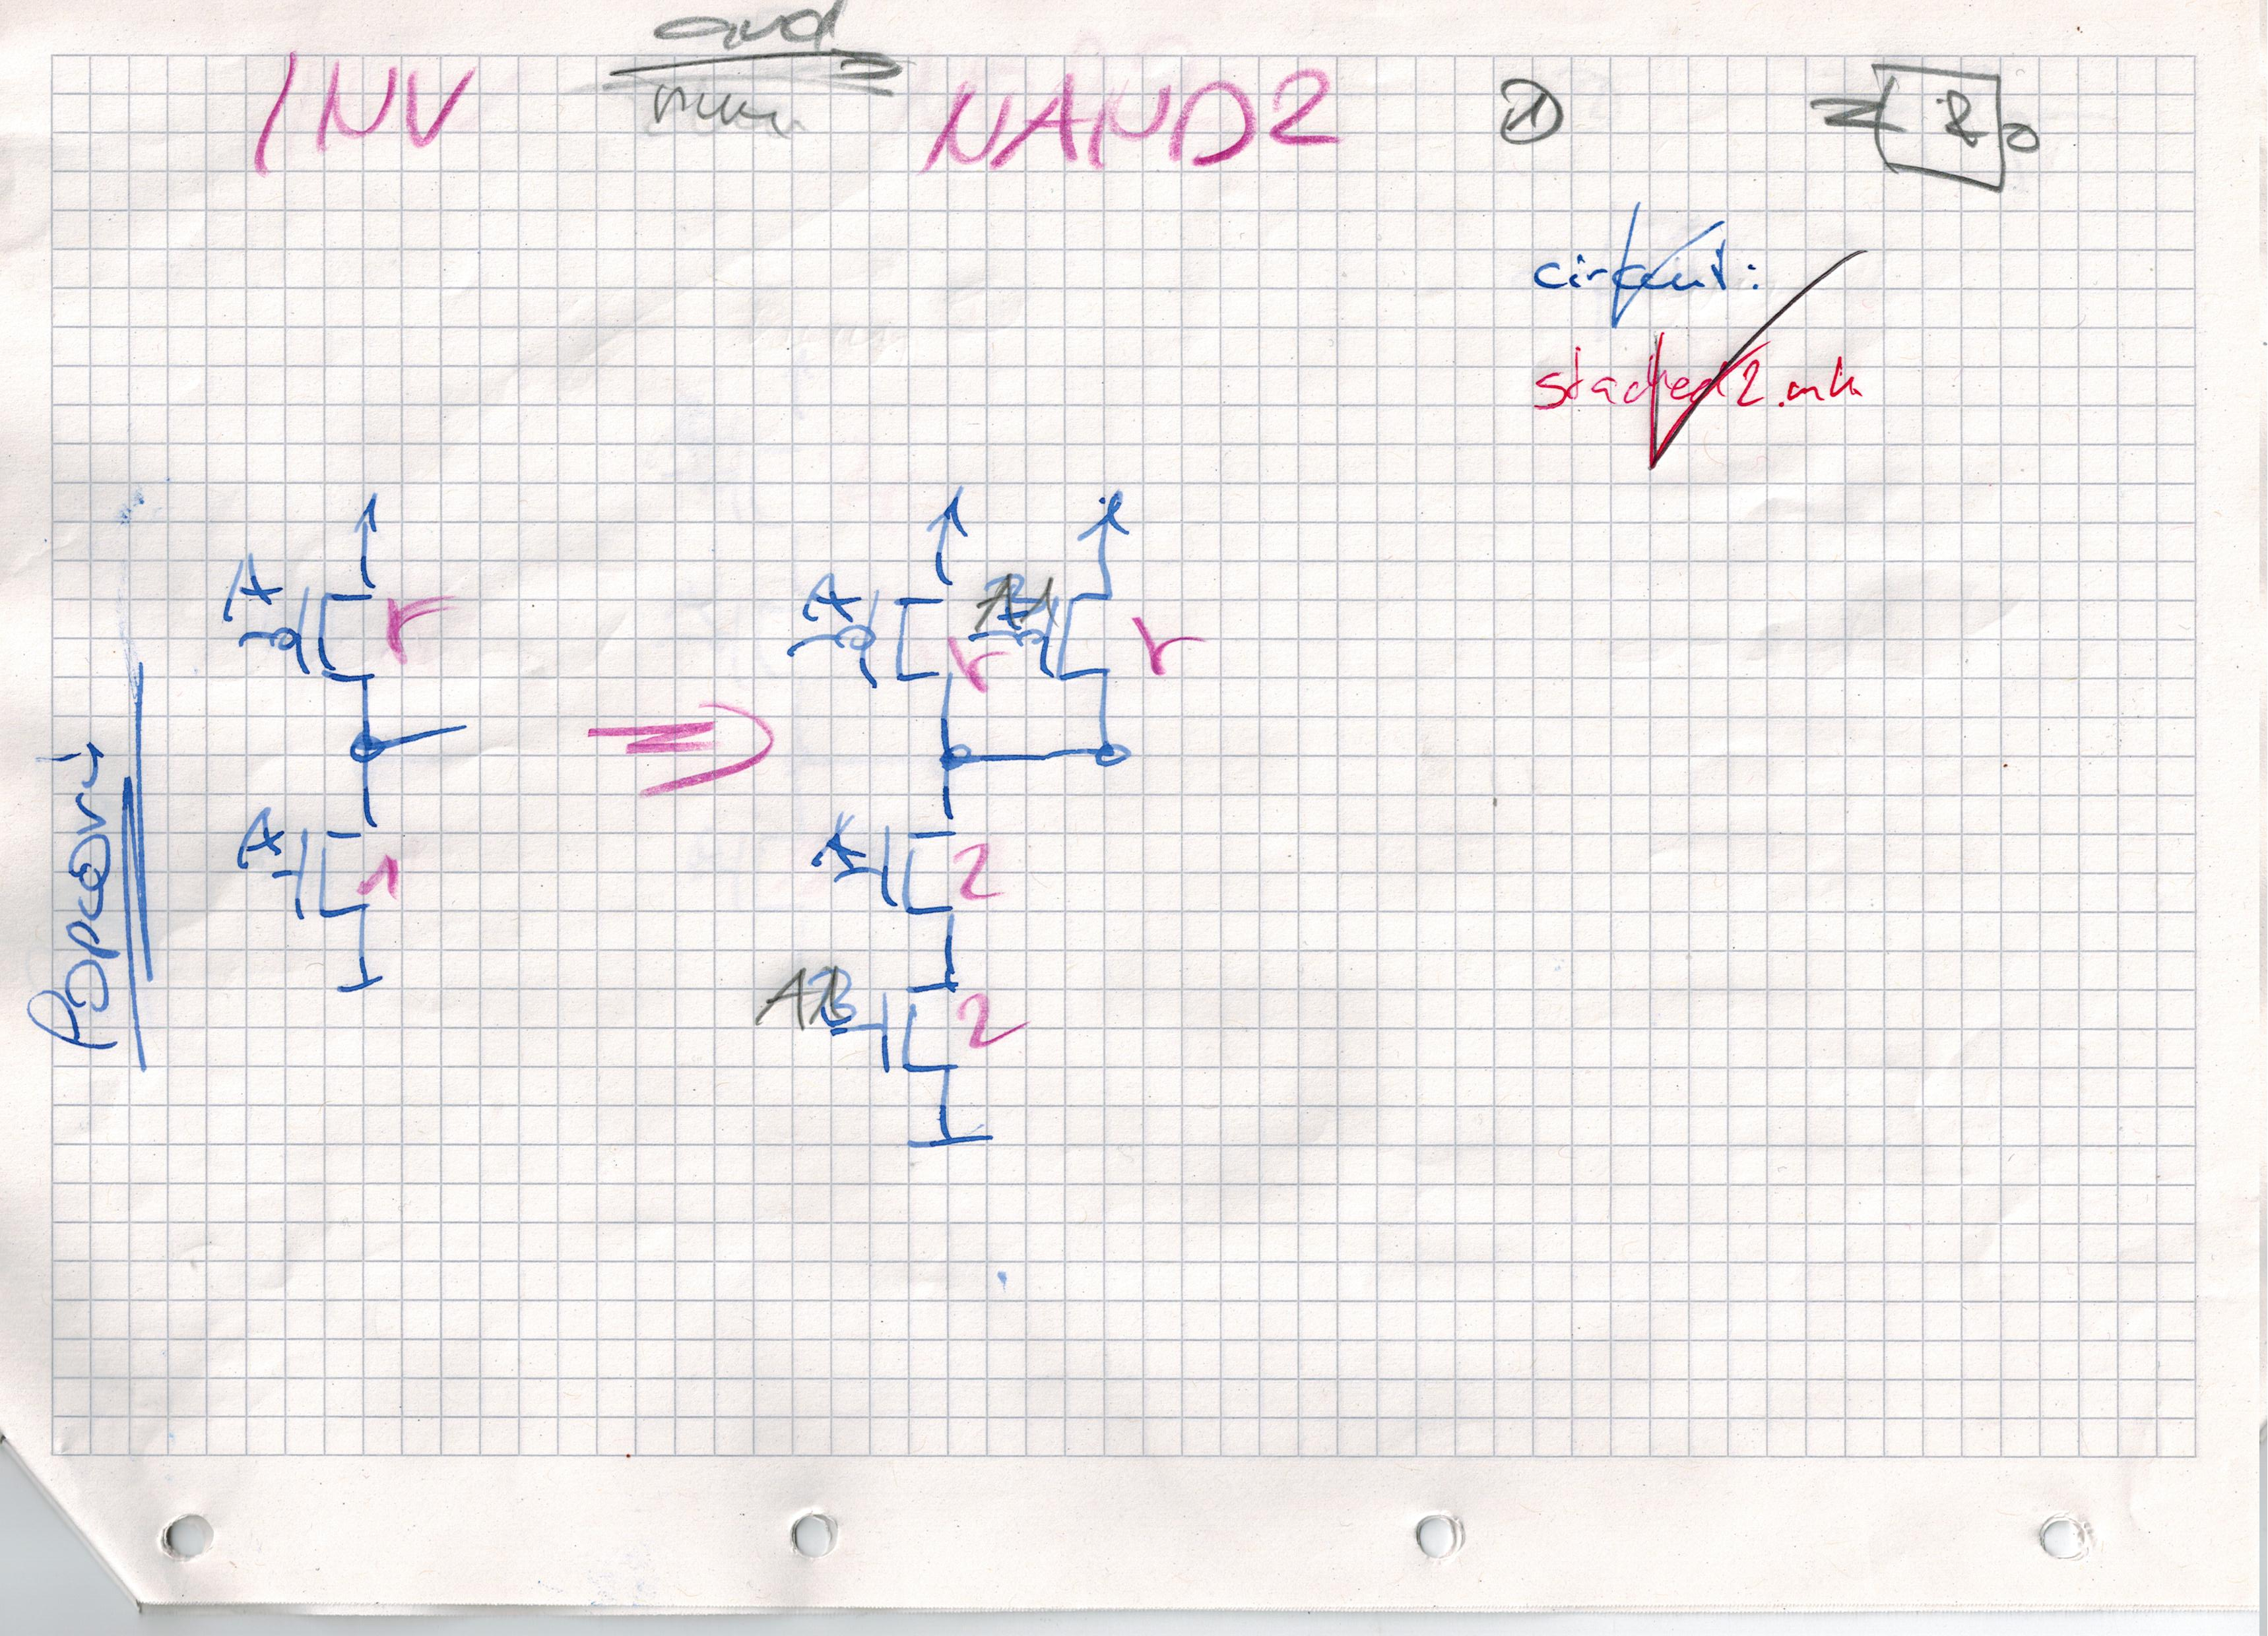
\includegraphics[width=0.85\textwidth]{NAND2.jpg}
    \end{center}
\end{frame}

%   ------------    aoaoaoi211111   -----------------------------------

\begin{frame}
\frametitle{AOAOAOI211111}
    \begin{center}
        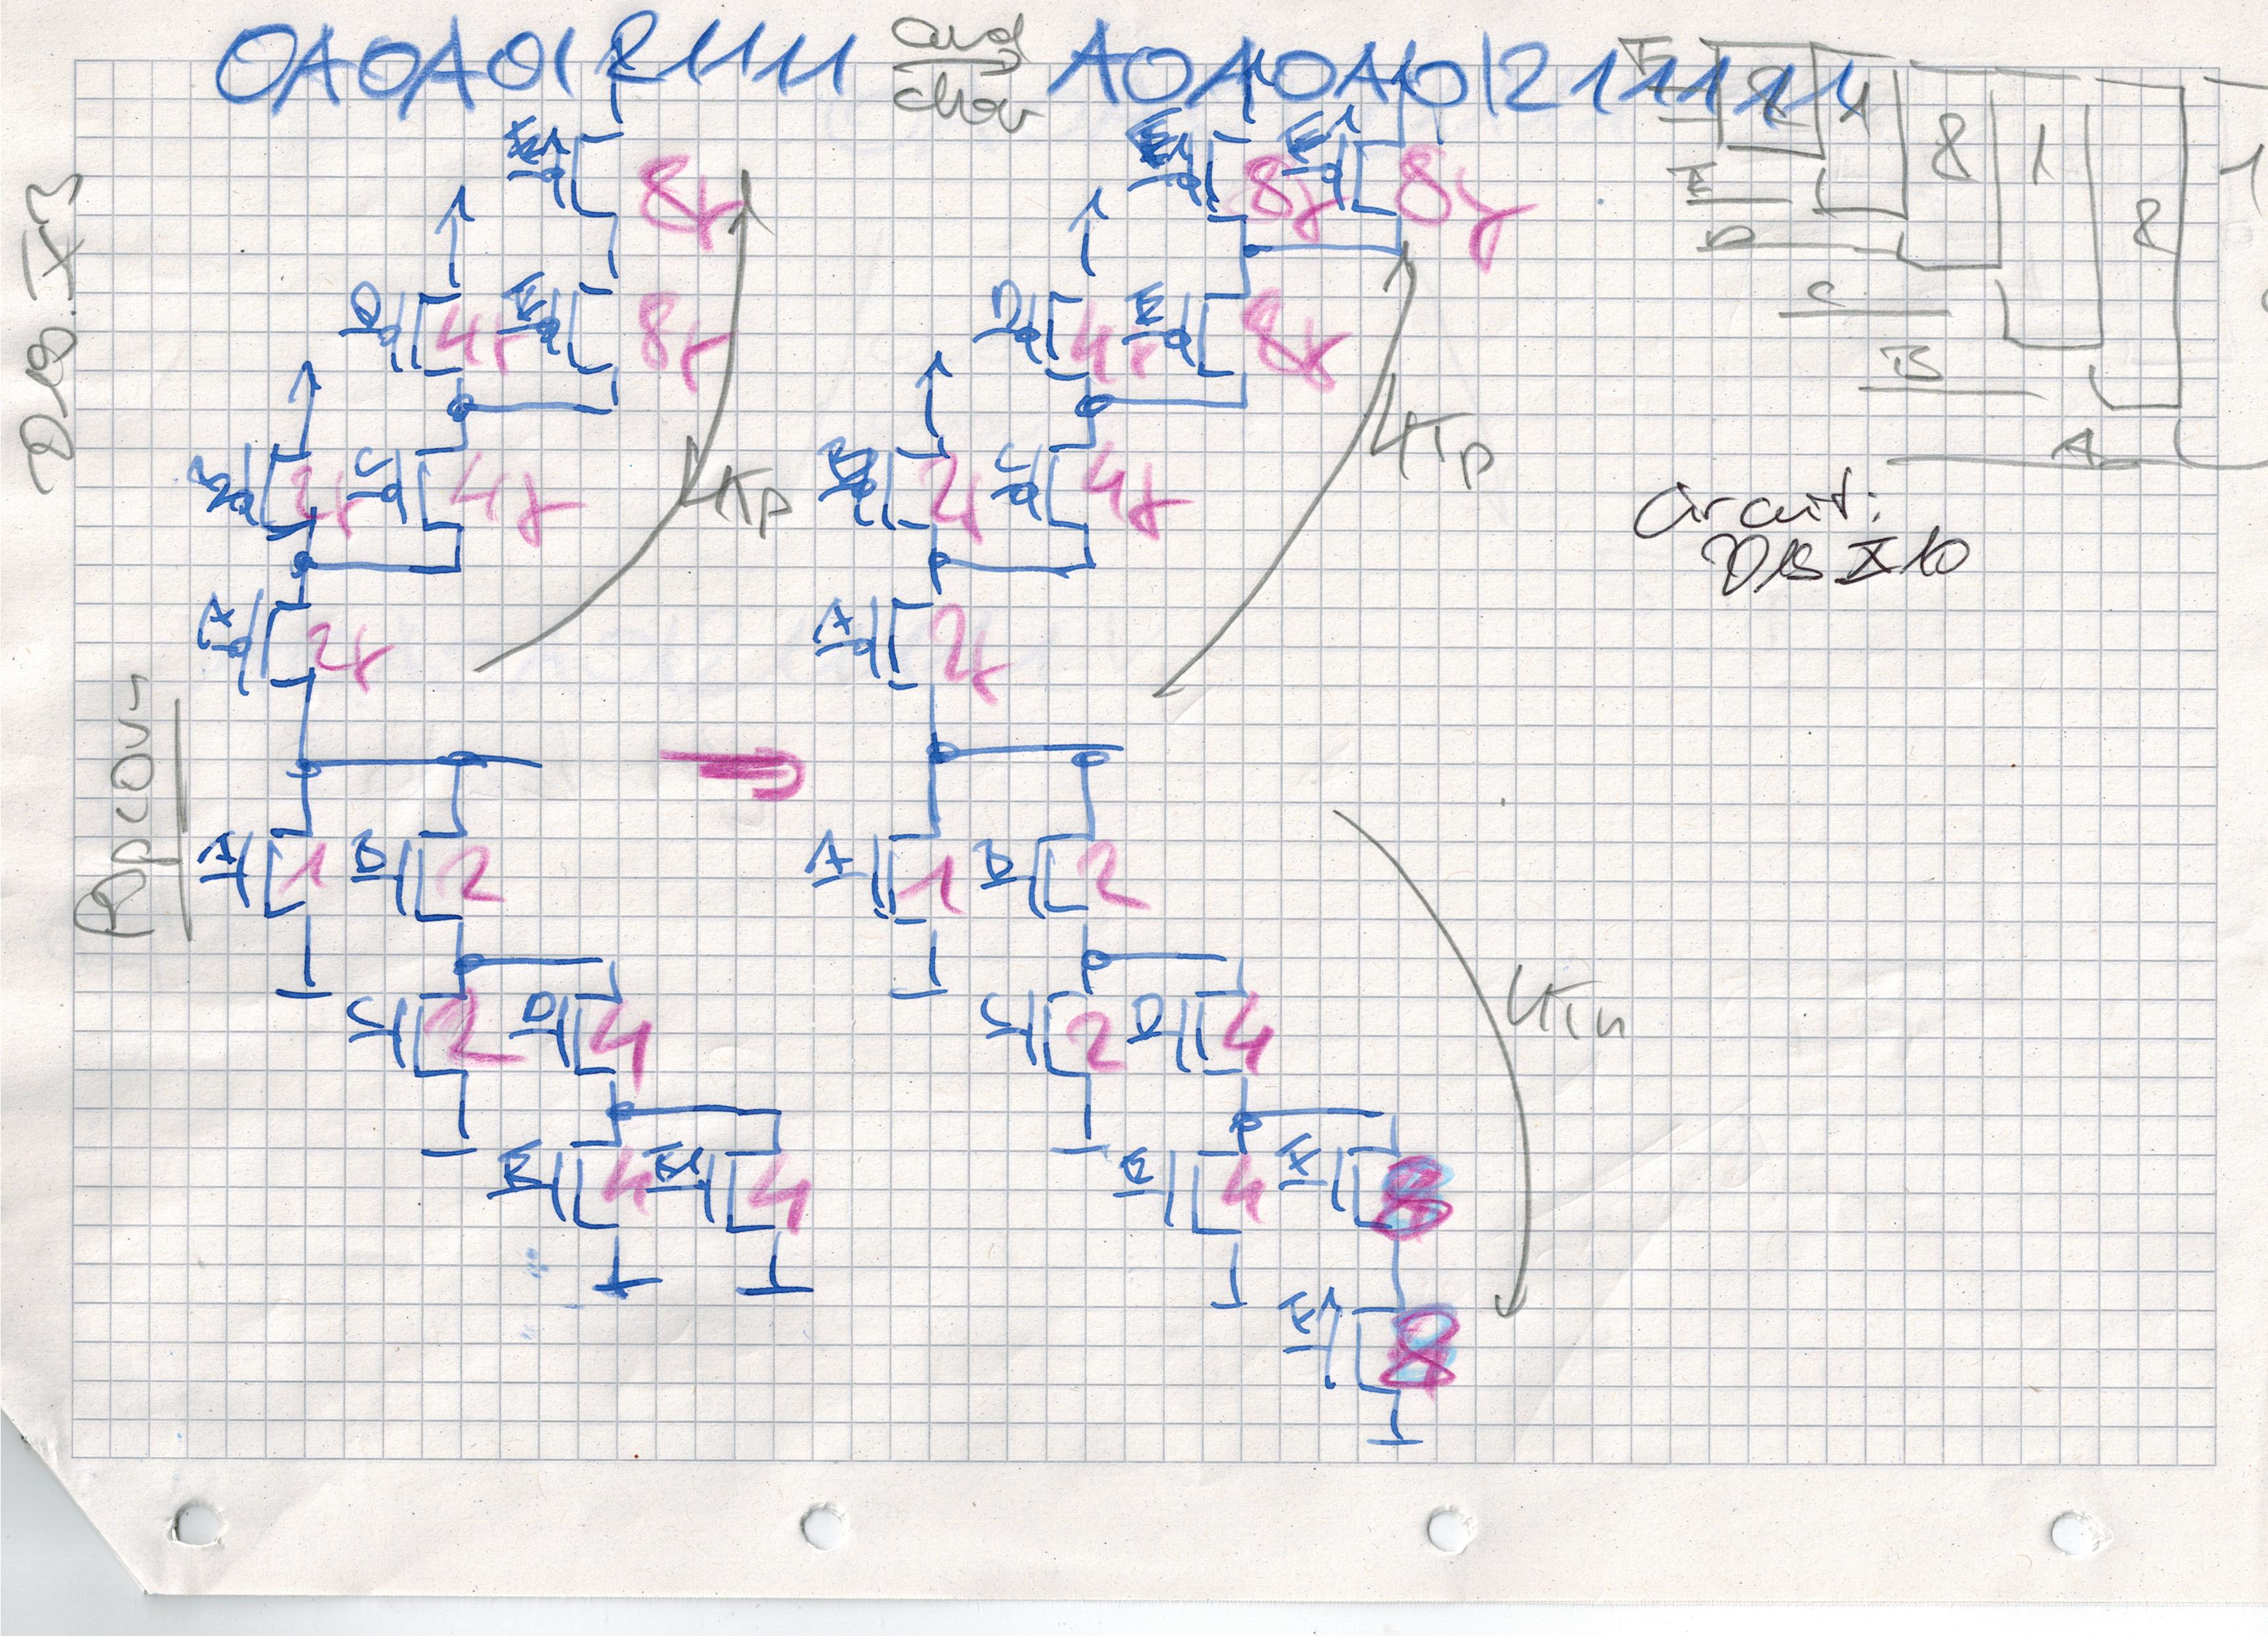
\includegraphics[width=0.85\textwidth]{AOAOAOI211111.jpg}
    \end{center}
\end{frame}

%   ------------    ooaaoaooai222112    -------------------------------

\begin{frame}
\frametitle{OOAAOAOOAI222112}
    \begin{center}
        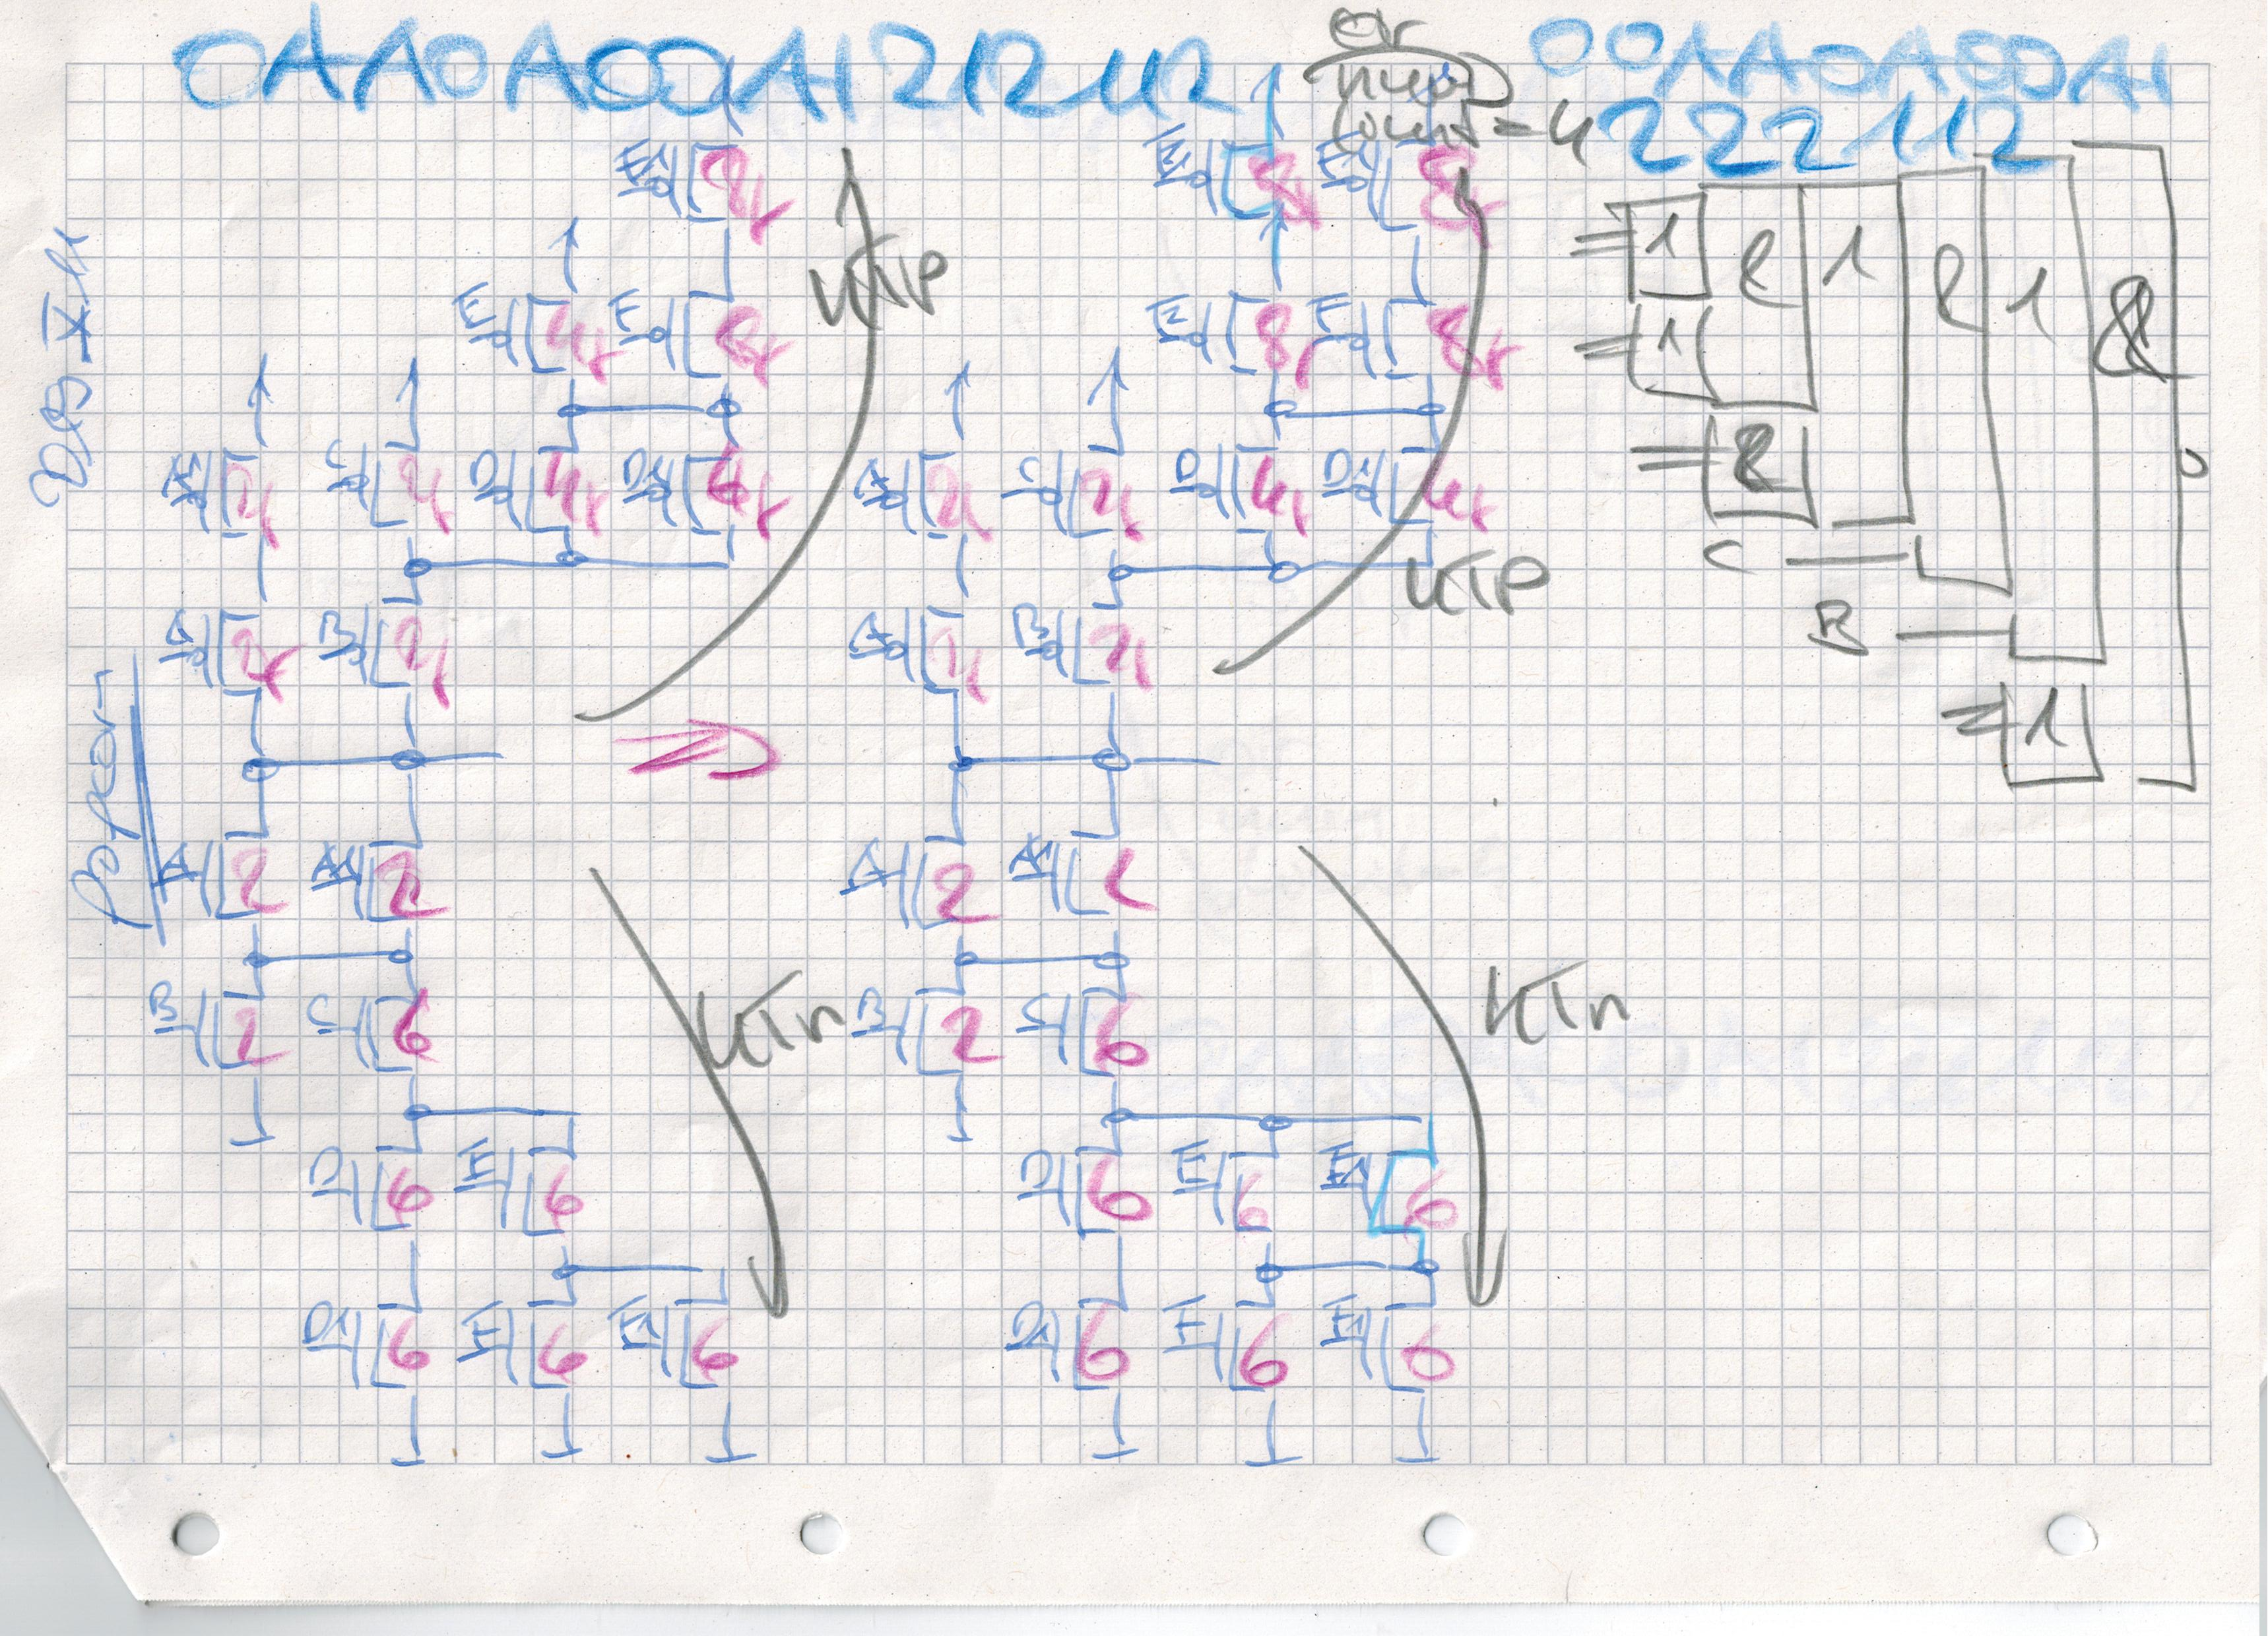
\includegraphics[width=0.85\textwidth]{OOAAOAOOAI222112.jpg}
    \end{center}
\end{frame}

%   ------------    paper work  ---------------------------------------

\begin{frame}
\frametitle{paper work}
    \begin{itemize}
%       \setlength\itemsep{1em}
        \item already done this for many, many complex gates
        \item currently 2 folder full of paper
        \item at least 500+ cells
        \item far from being complete
    \end{itemize}
program a piece of software for help
\end{frame}

%   ===================================================================
\section{Popcorn}
%   ===================================================================

%   ------------    man pages   ---------------------------------------

\begin{frame}
\frametitle{manual pages}
    \texttt{\% make tools}
    \newline
    \texttt{\% evince -s Tools/popcorn.1.ps}
    \newline
    \texttt{\% evince -s Tools/cell.5.ps}
\end{frame}

%   ------------    principle   ---------------------------------------

\begin{frame}
\frametitle{principle}
    \begin{center}
        \begin{tikzpicture}[node distance = 2cm, auto]
            \node [block] (tool) {popcorn -m};
            \node [cloud, left of=tool] (filein) {cell\_file};
            \node [cloud, right of=tool] (fileout) {cell\_file};
            \path [line,dashed] (filein) -- (tool);
            \path [line,dashed] (tool) -- (fileout);
        \end{tikzpicture}
    \end{center}
    \texttt{\% popcorn -l 2 -b 3}
    \texttt{\textcolor{green}{-m nor}}
    \texttt{-c NOR2 Catalog/INV > Catalog/NOR2}
    \newline
    \texttt{\% popcorn -l 2}
    \texttt{\textcolor{blue}{-b 3} \textcolor{green}{-m nand}}
    \texttt{-c NAND2 Catalog/INV > Catalog/NAND2}
    \newline
    \texttt{\% popcorn -l 2}
    \texttt{\textcolor{blue}{-b 2}}
    \texttt{-m nand -c AND2 Catalog/INV > Catalog/AND2}
\end{frame}

%   ------------    hand-crafted cells  -------------------------------

\begin{frame}
\frametitle{LATP}
    \begin{center}
        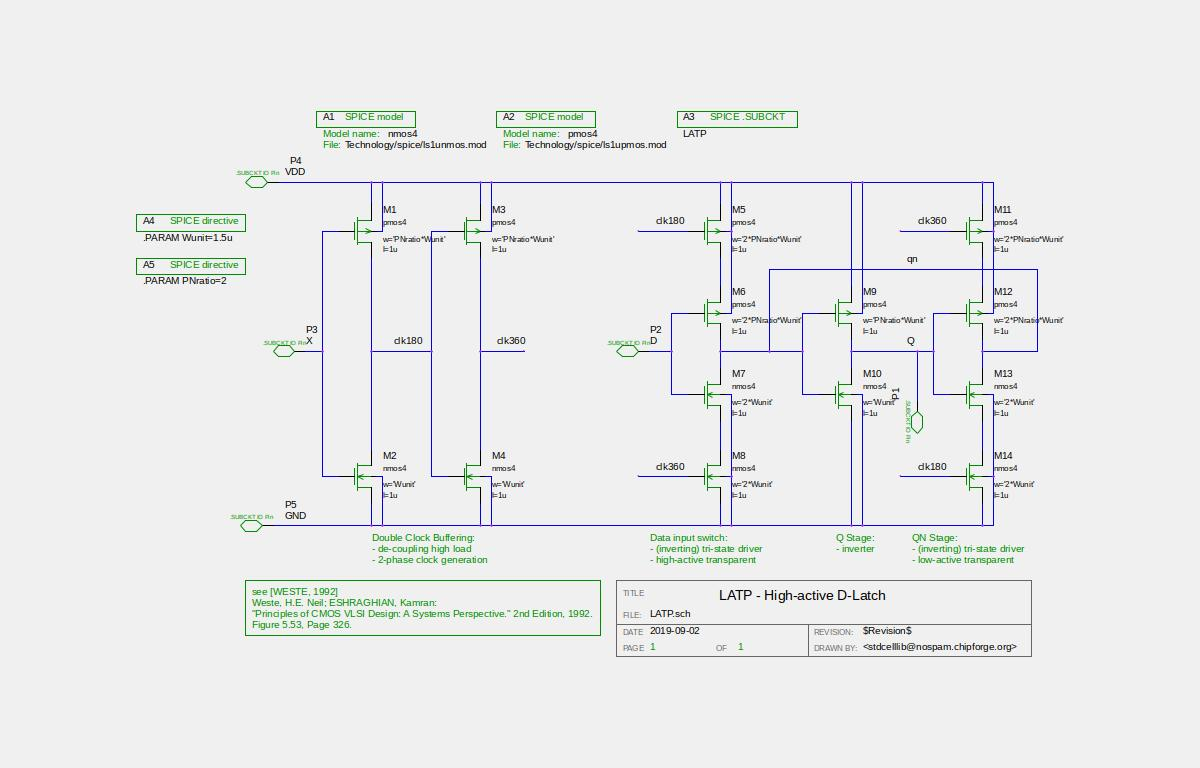
\includegraphics[width=0.85\textwidth]{LATP.jpeg}
    \end{center}
\end{frame}

\begin{frame}
\frametitle{LATN}
    \begin{center}
        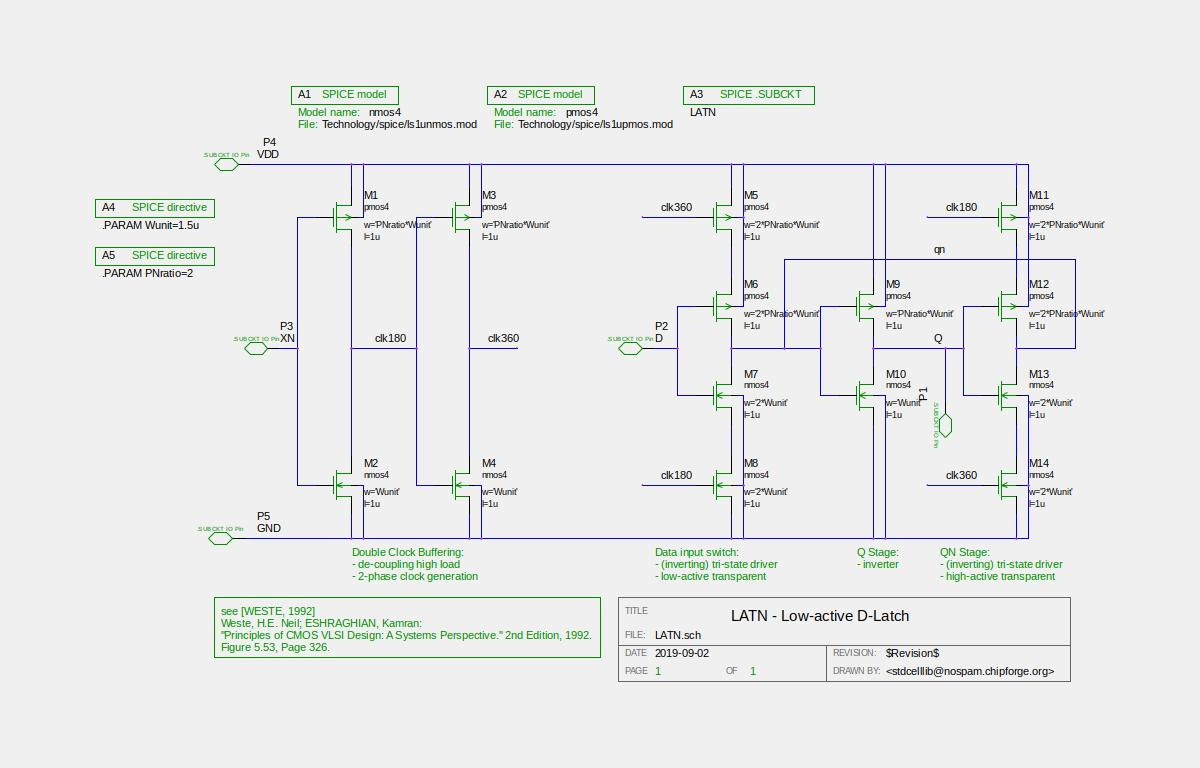
\includegraphics[width=0.85\textwidth]{LATN.jpeg}
    \end{center}
\end{frame}

\begin{frame}
\frametitle{LATERP}
    \begin{center}
        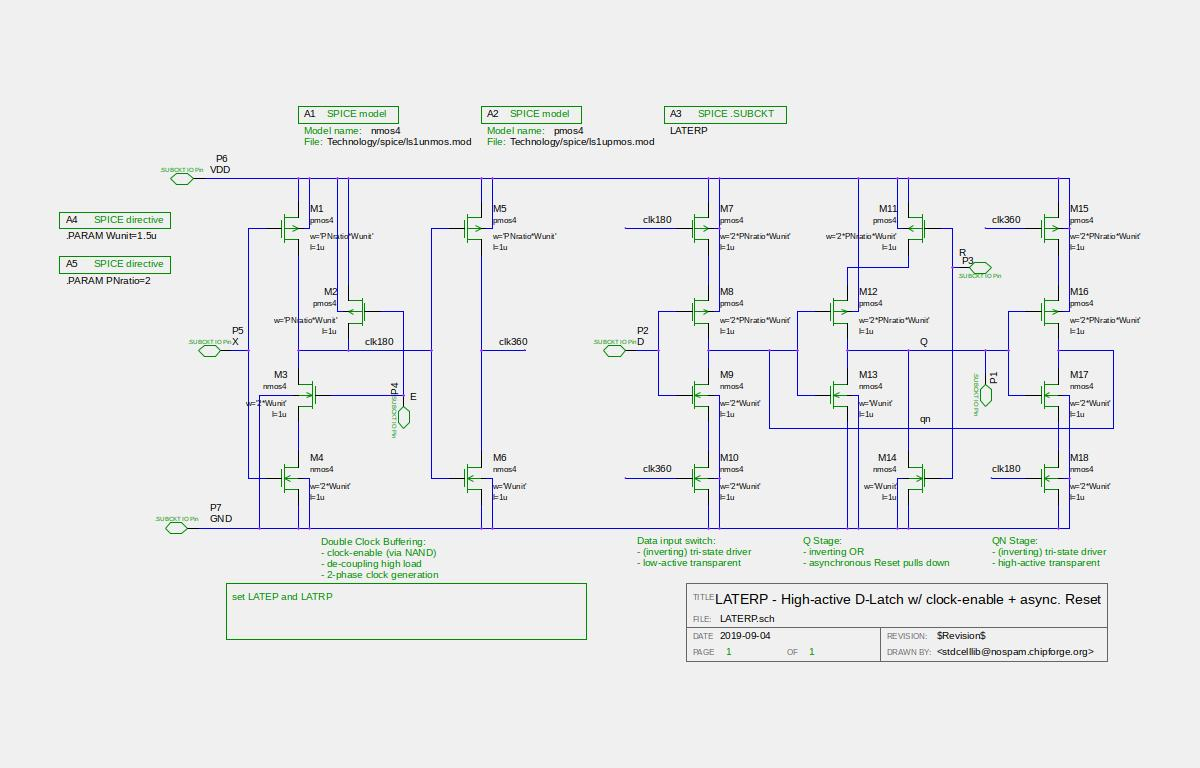
\includegraphics[width=0.85\textwidth]{LATERP.jpeg}
    \end{center}
\end{frame}

%   ------------    to do   -------------------------------------------

\begin{frame}
\frametitle{to do}
    \begin{center}
        \begin{tikzpicture}[node distance = 2cm, auto]
            \node [block] (tool) {netlister};
            \node [cloud, left of=tool] (filein) {schematic};
            \node [cloud, right of=tool] (fileout) {cell\_file};
            \path [line,dashed] (filein) -- (tool);
            \path [line,dashed] (tool) -- (fileout);
        \end{tikzpicture}
    \end{center}
    for hand-crafted cells
    \bluebox{NOTE:}{not yet implemented}
\end{frame}

%   ===================================================================
\section{Catalog}
%   ===================================================================

%   ------------    'ls -1 Catalog/*'   -------------------------------

\begin{frame}
\frametitle{'ls -1 Catalog/*'}
    \texttt{Catalog/INV}
    \newline
    \texttt{Catalog/stacked2\_cells.mk}
    \newline
    \texttt{Catalog/stacked3\_cells.mk}
    \newline
    \texttt{Catalog/stacked4\_cells.mk}
    \newline
    \texttt{Catalog/GNUmakefile}
\end{frame}

%   ------------    'make catalog"  -----------------------------------

\begin{frame}
\frametitle{'make catalog'}
    \bluebox{WARNING:}{at your own risk}
\end{frame}

%   ------------    help    -------------------------------------------

\begin{frame}
\frametitle{help screen}
    \texttt{\% make}
    \newline
    or
    \newline
    \texttt{\% make help}
\end{frame}

%   ===================================================================
\section{Layout}
%   ===================================================================

%   ------------    mosis   -------------------------------------------

\begin{frame}
\frametitle{MOSIS design rules}
    \begin{itemize}
        \item \texttt{https://en.wikipedia.org/wiki/MOSIS}
        \item U.S. University program for chip design
        \item defines common design rules, feasible for almost all technologies
        \item running Multi-project Wafers
        \item similiar to Europractice in the EU
    \end{itemize}
\end{frame}

%   ------------    'mosis-rules.scm'   -------------------------------

\begin{frame}
\frametitle{'less Tools/popcorn/mosis-rules.scm'}
coded for
    \newline
    \begin{itemize}
        \item SCMOS: scalable CMOS technologies
        \item SUBM:  sub-micron CMOS technologies ($\leq 0.8 \mu$)
        \item DEEP:  deep sub-micron CMOS technologies ($\leq 0.35 \mu$)
        \item USER:  reserved for future, loadable design rule values
    \newline
        \item all rules in $\lambda$
        \item $1 \lambda$ is half the 'feature size' of a technology node
        \item hence 'scalable'
    \end{itemize}
\end{frame}

%   ------------    T6_NAND2    ---------------------------------------

\begin{frame}
\frametitle{T6\_NAND2}
    \begin{center}
        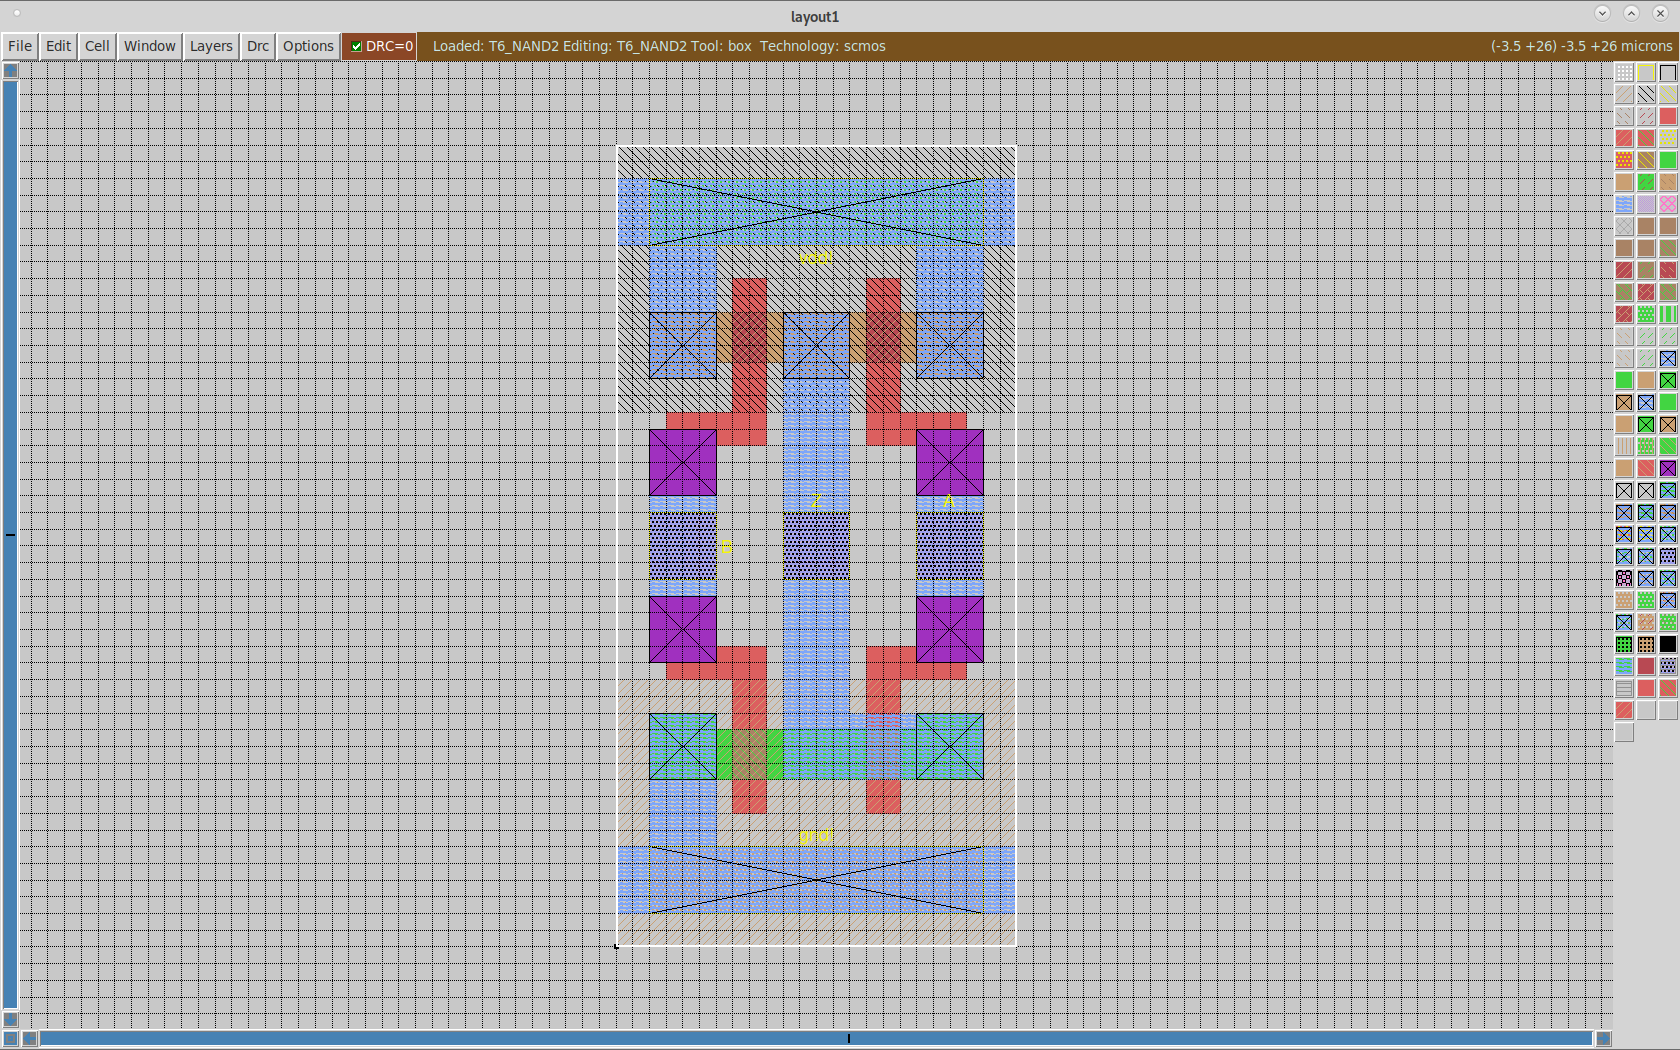
\includegraphics[width=0.8\textwidth]{T6_NAND2.png}
    \end{center}
6 Metal tracks
\end{frame}

%   ------------    T7_NAND2    ---------------------------------------

\begin{frame}
\frametitle{T7\_NAND2}
    \begin{center}
        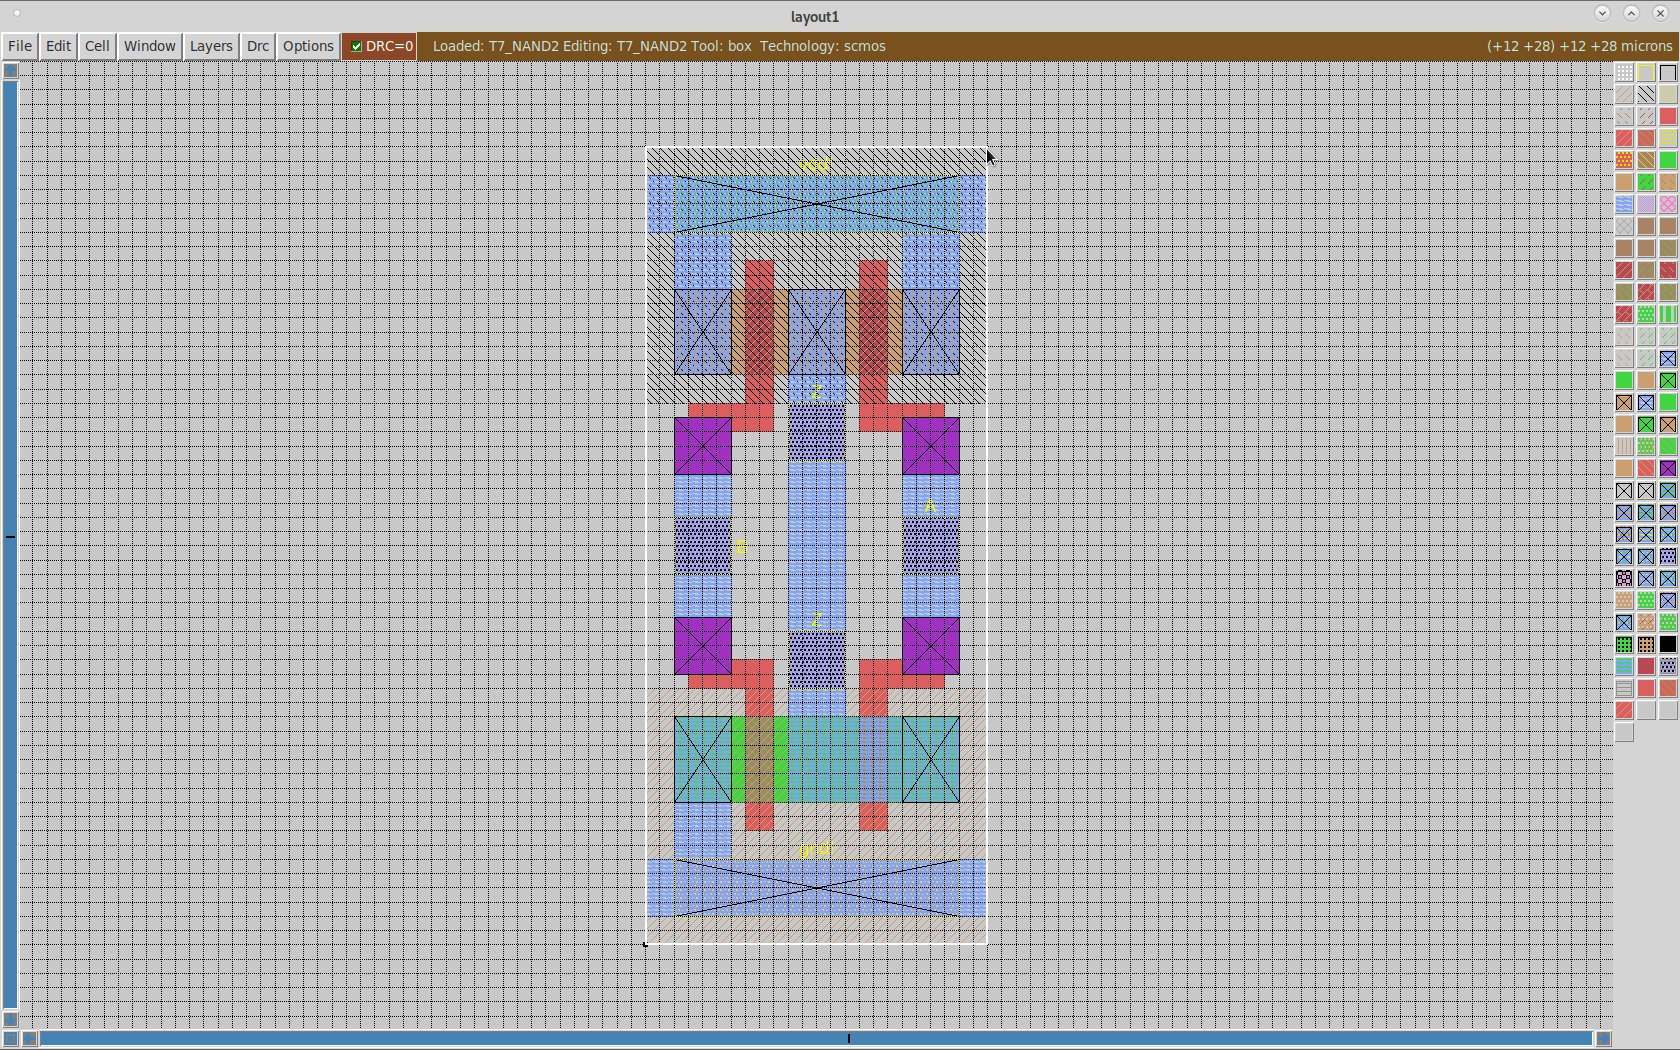
\includegraphics[width=0.8\textwidth]{T7_NAND2.png}
    \end{center}
7 Metal tracks
\end{frame}

%   ------------    T10_NAND2   ---------------------------------------

\begin{frame}
\frametitle{T10\_NAND2}
    \begin{center}
        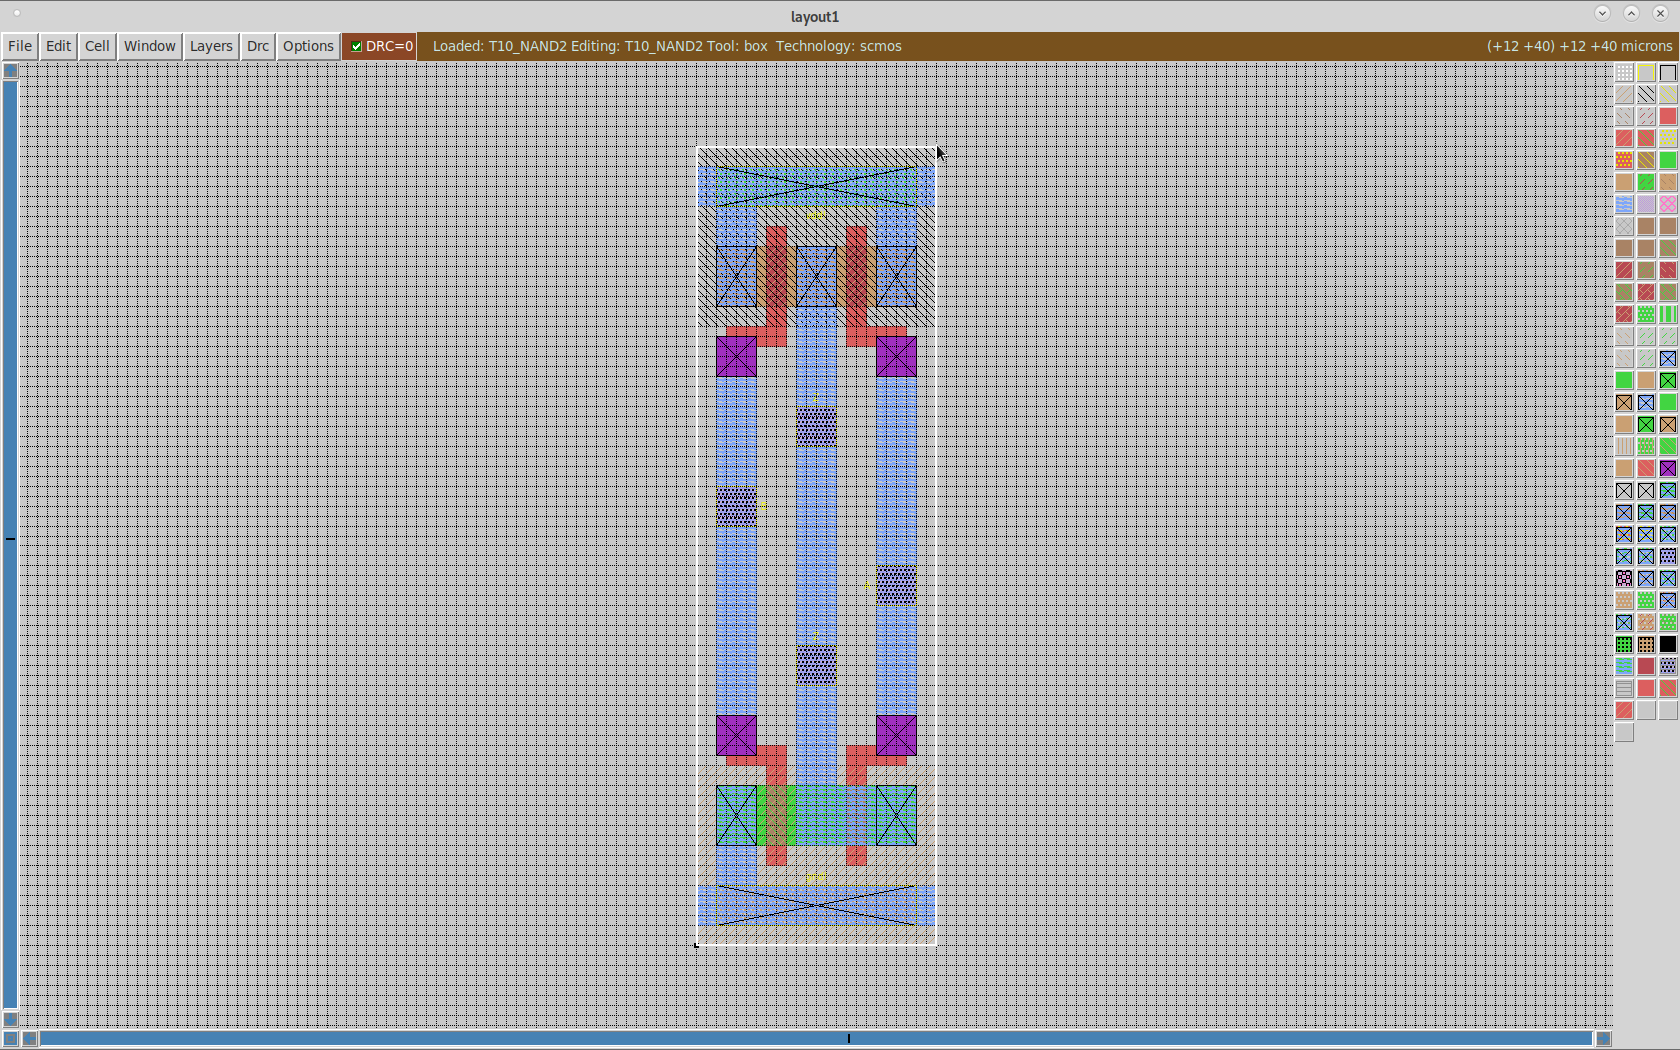
\includegraphics[width=0.8\textwidth]{T10_NAND2.png}
    \end{center}
10 Metal tracks
\end{frame}

%   ===================================================================
\section{Configuration}
%   ===================================================================

%   ------------    TOML    -------------------------------------------

\begin{frame}
\frametitle{'less Templates/TOML/LS1u\_std.toml'}
\end{frame}

%   ------------    one day     ---------------------------------------

\begin{frame}
\frametitle{one day in the future you can}
    \begin{itemize}
        \item configure TOML file
        \item typing \texttt{\% make dist} \newline
        \item all schematics are generated from cell files
        \item all layouts are generated from cell files
        \item runs spice, extract timing / propagation delays
        \item generate liberty file format for 'yosys'
        \item generate data sheets
        \item get your free and open source Standard Cell Library
    \end{itemize}
\end{frame}

%   ===================================================================
\section{End}
%   ===================================================================

%   ------------    end     -------------------------------------------

\begin{frame}{End}
    \begin{center}
        \textbf{Mailing List:} \url{https://list.libresilicon.com/mailman/listinfo/libresilicon-developers}
    \end{center}
    \vfill
    \begin{center}
        \textbf{Danke für Ihre Aufmerksamkeit!} \\
        \textbf{Thanks your attention!} \\
    \end{center}
\end{frame}

%   ------------    over    -------------------------------------------

\begin{frame}
    \begin{itemize}
        \item from cell file to schematic ($\rightarrow$ still broken)
        \item from cell file to layout ($\rightarrow$ over engineered, needs rebuild)
        \item from cell file to spice ($\rightarrow$ rebuild?)
        \item from spice simulation to timing ($\rightarrow$ with issues)
        \item generating liberty file format for 'yosys' ($\rightarrow$ still open)
        \item and than - data sheets generation
    \end{itemize}
\end{frame}

\end{document}
